\subsection{Begriffserkl"arungen}

\begin{figure*}[b]
	\centering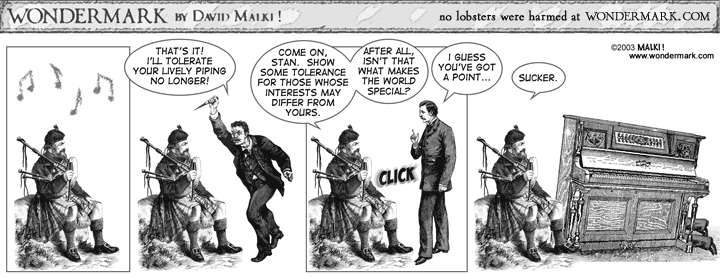
\includegraphics[width=0.9\textwidth]{bilder/comics/wondermark003.png}
\end{figure*}

% TODO sind die Begriffe, die man für den Studienplan braucht, hier gut untergebracht oder sollten die mit in den restlichen Erklärungstext? Ist das hier wirklich eine kurze, neutrale Begriffserklärung oder nicht eher ein Kapitel "Kritische Kommentrare zu den Vorlesungen und Übungen"?

Einen guten "Uberblick "uber die an der Uni gebr"auchlichen Begriffe und
Abk"urzungen findest du im "`Uni-ABC"' des AStA-Erstiinfos. Im folgenden
sind nur die wichtigen Begriffe f"ur deinen Stundenplan erkl"art, den du
auf der letzten Seite dieses Heftes findest.


\subsubsection*{Vorlesung}

Vorlesungen werden vom Professor vor allen Studis abgehalten und befassen
sich in erster Linie mit der theoretischen Herleitung des Stoffes. Teilweise
sind Vorlesungen aber auch nur mehr oder weniger interessante Folienfilme auf
dem Overhead-Projektor. Solltest du in der Vorlesung einmal etwas nicht
verstehen, so ist das nicht so tragisch, den meisten deiner Kommilitonen geht
es nicht anders. Schau dich mal um und du wirst viele andere fragende Gesichter
sehen\ldots Du darfst nicht damit rechnen, wie in der Schule, das meiste sofort zu
verstehen, f"ur jede Vorlesung sollte man eine gewisse Nacharbeitungszeit
einplanen. In einer Vorlesung ist wegen der gro"sen Teilnehmerzahl
normalerweise kein Dialog mit dem Vortragenden m"oglich. Aufgetretene Fragen
k"onnen und sollten am besten direkt nach der Vorlesung oder sonst in einer
Sprechstunde mit dem Professor gekl"art werden.


\subsubsection*{Gro"se "Ubung}

Erg"anzend gibt es die gro"sen "Ubungen, auch Saal"ubungen genannt. Diese
finden~-- wie die Vorlesung~-- vor dem gesamten Auditorium statt und sollen das
(vielleicht) erworbene theoretische Wissen vertiefen und vor allem auch
praktische, klausurbezogene Anwendungen aufzeigen. Die gro"se "Ubung wird
normalerweise von einem Assistenten gehalten, selten vom Professor selbst.
Assistenten ("`Assis"') sind fertige Dipl.-Ings, Dipl.Informs etc. und sind
Angestellte des Instituts, aus dem auch der jeweilige Professor stammt. Die
Assis sind bei fachlichen Fragen kompetente Ansprechpartner und meist auch sehr
hilfsbereit. Da Assistenten "ublicherweise die Klausuren entwerfen, kann man
bei genauem Hinh"oren in den gro"sen "Ubungen oder im privaten Gespr"ach mit
dem Assi einiges "uber den Tag der Wahrheit erfahren.


\subsubsection*{Kleine "Ubung, Seminargruppe}

Als erstes eine Warnung: Kleine "Ubungen tauchen in deinem Stundenplan nicht auf!
Also f"ull bitte nicht alle L"ucken im
Stundenplan mit Sprachkursen, Sportveranstaltungen und Klavierunterricht auf,
sondern lass noch ein bisschen Platz. Leider werden kleine "Ubungen nur in
einigen F"achern angeboten. Der Begriff Seminargruppe ist synonym zu verstehen.
In kleinen "Ubungen soll man eigentlich selbst Aufgaben l"osen. Dies geschieht
unter Anleitung der HiWis (Hilfswissenschaftler), welche besonders qualifizierte
(!?) Studierende h"oheren Semesters sind. F"ur die kleinen "Ubungen werden die
Studis in etwa 20- bis 30-k"opfige Gruppen aufgeteilt. Hierbei ist darauf zu
achten, rechtzeitig zum Termin zur Gruppeneinteilung zu erscheinen, um diese
Veranstaltungen m"oglichst g"unstig im Stundenplan positionieren zu k"onnen.
Manche Assistenten haben inzwischen auch Methoden entwickelt, bei denen man
ohne Ellenbogen einen passenden Termin bekommt, aber das hat sich noch nicht
vollst"andig durchgesetzt. Aufgrund der geringen Teilnehmerzahlen ist in
kleinen "Ubungen der Dialog mit dem Vortragenden m"oglich und sinnvoll. Wenn
man einen guten HiWi erwischt hat, dann kann man in den kleinen "Ubungen all
die Wissensl"ucken auff"ullen, die nach Vorlesung und gro"ser "Ubung noch offen
sind.

% TODO Spätestens hier (Noch Fragen?) hört's auf, die Fragen sind keine Begriffsklärung mehr. Das ist ja gut, dass es solche Texte gibt, aber die Überschrift passt einfach nicht.
\subsubsection*{Noch Fragen?}

Die Qualit"at dieser drei Veranstaltungsarten ist in starkem Ma"se vom
jeweiligen Vortragenden abh"angig. W"ahrend du unter Umst"anden die
Seminargruppen noch wechseln kannst, so ist das bei den erstgenannten
Veranstaltungen nat"urlich nicht m"oglich.

Du wirst sehr bald feststellen, dass es verschiedene Lerntypen gibt. Manche
deiner Kommilitonen werden kaum eine Vorlesung besuchen, sondern stattdessen die gro"sen
und kleinen "Ubungen verschlingen. Wieder andere lassen sich sowieso kaum im
H"orsaal blicken, sondern k"onnen am besten zu Hause oder in der Uni-Bibliothek
autodidaktisch lernen.

Wenn trotz Vorlesungen, gro"ser "Ubungen und kleiner "Ubungen noch Fragen
auftreten, so hilft dir das Gespr"ach mit den Kommilitonen oder der Blick in
entsprechende Literatur.
Wichtig: Kaufe nicht gleich jedes empfohlene Buch neu,
das ist Geldverschwendung. Frage h"ohere Semester nach wirklich sinnvoller
Literatur, leih' dir die B"ucher aus der UB aus, gebrauchte B"ucher gibt es
g"unstig z.B. in der Newsgroup \nurl{http://groups.google.de/group/braunschweig.kaufrausch/} (siehe den Artikel
ab Seite \pageref{elekinf}). An der Uni wird man nicht umsorgt wie etwa in der
Schule oder in der betrieblichen Ausbildung, du tr"agst ein wesentlich h"oheres
Ma"s an Eigenverantwortung. Zur Orientierung in der ersten Zeit ist ein
Ansprechpartner unentbehrlich. Wenn die Kommilitonen aus
deinem eigenen Semester nicht weiterhelfen k"onnen, dann vielleicht dein/e TutorIn oder andere
Studierende im h"oheren Semester (zum Beispiel Mitbewohner, Fachgruppe).
